\documentclass[10pt, a4paper]{article}
\usepackage{subfiles}

\usepackage[T1]{fontenc}
\usepackage[utf8]{inputenc}
\usepackage[italian]{babel}

\usepackage{pdfpages}
\usepackage{youngtab}
\usepackage{physics}
\usepackage{tikz}
\usepackage{amsmath}
\usepackage{amssymb}
\usepackage{amsthm}
\usepackage{siunitx}
\newcommand*\chem[1]{\ensuremath{\mathrm{#1}}}
\usepackage[margin=1.00in]{geometry}
\usepackage{lmodern}

\theoremstyle{plain} 
\newtheorem{ese}{Esercizio}

\newenvironment{svol}{\paragraph{Svolgimento:}}{\hfill$\square$\newline}

\newcommand{\der}[3][]{\ensuremath{\dfrac{d^{#1}#2}{d#3^{#1}}}}

\newenvironment{dati}{\paragraph{Dati:}}{\hfill}

\begin{titlepage}
	\title{Esercizi del corso di Istituzioni di Fisica Nucleare e Subnucleare}
	\author{Davide Passaro \\ Matricola: 867815}
	\date{}
\end{titlepage}

\begin{document}
	\maketitle
	\section{Fisica nucleare}
		\subfile{SubFiles/Radioattività.tex}
		\subfile{SubFiles/DecadimentiAlpha.tex}
		\subfile{SubFiles/Fissione.tex}
		\subfile{SubFiles/ShellModel.tex}

	\section{Fisica delle particelle}
		\subfile{SubFiles/BetaDecay.tex}
		\subfile{SubFiles/NuclearFusion.tex}
		\subfile{SubFiles/EtaDecay.tex}
		\subfile{SubFiles/QuarkModel.tex}

	\section{Conti}
		Per gli esercizi per i quali è stato necessario fare dei conti è stato usato il software Mathematica. I fogli di calcolo utilizzati sono elencati in seguito esercizio per esercizio.
		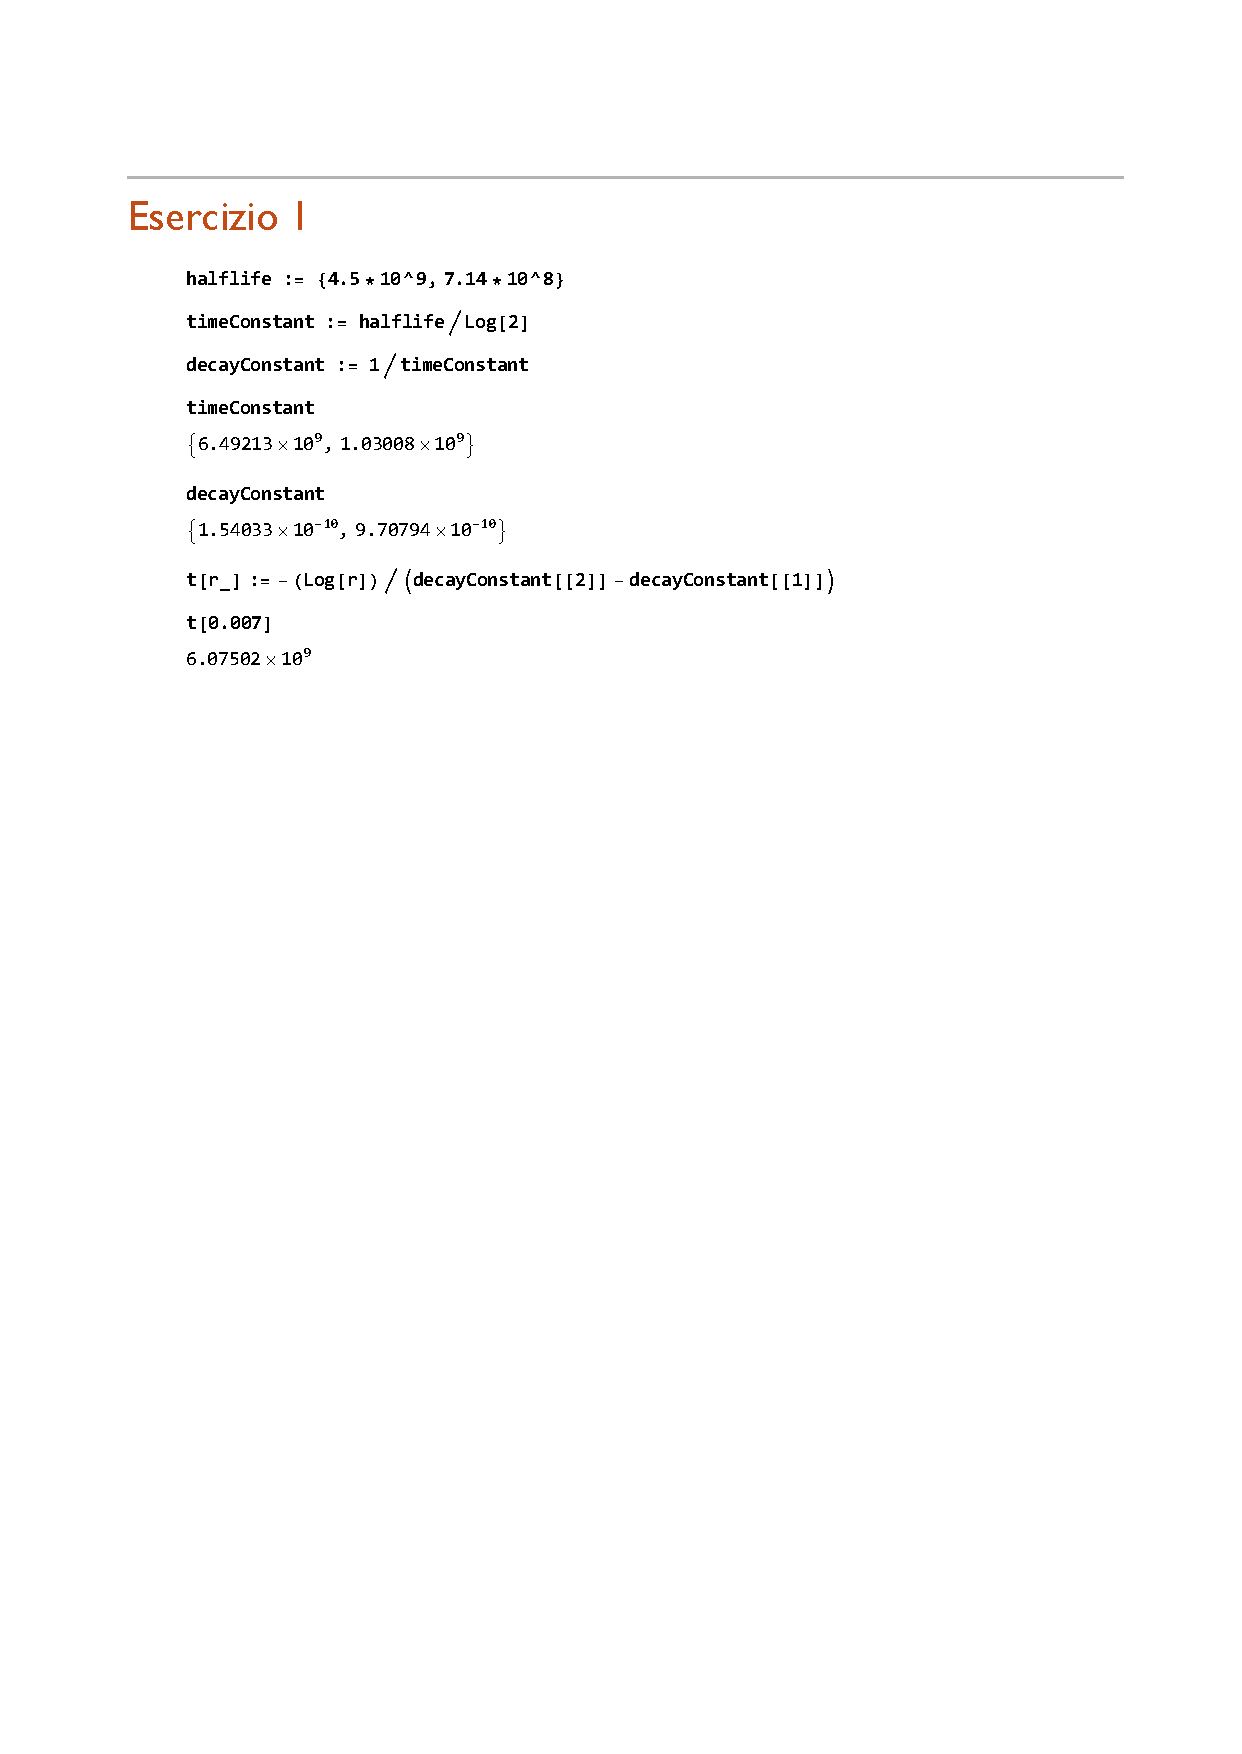
\includepdf{Conti/Esercizio1.pdf}
		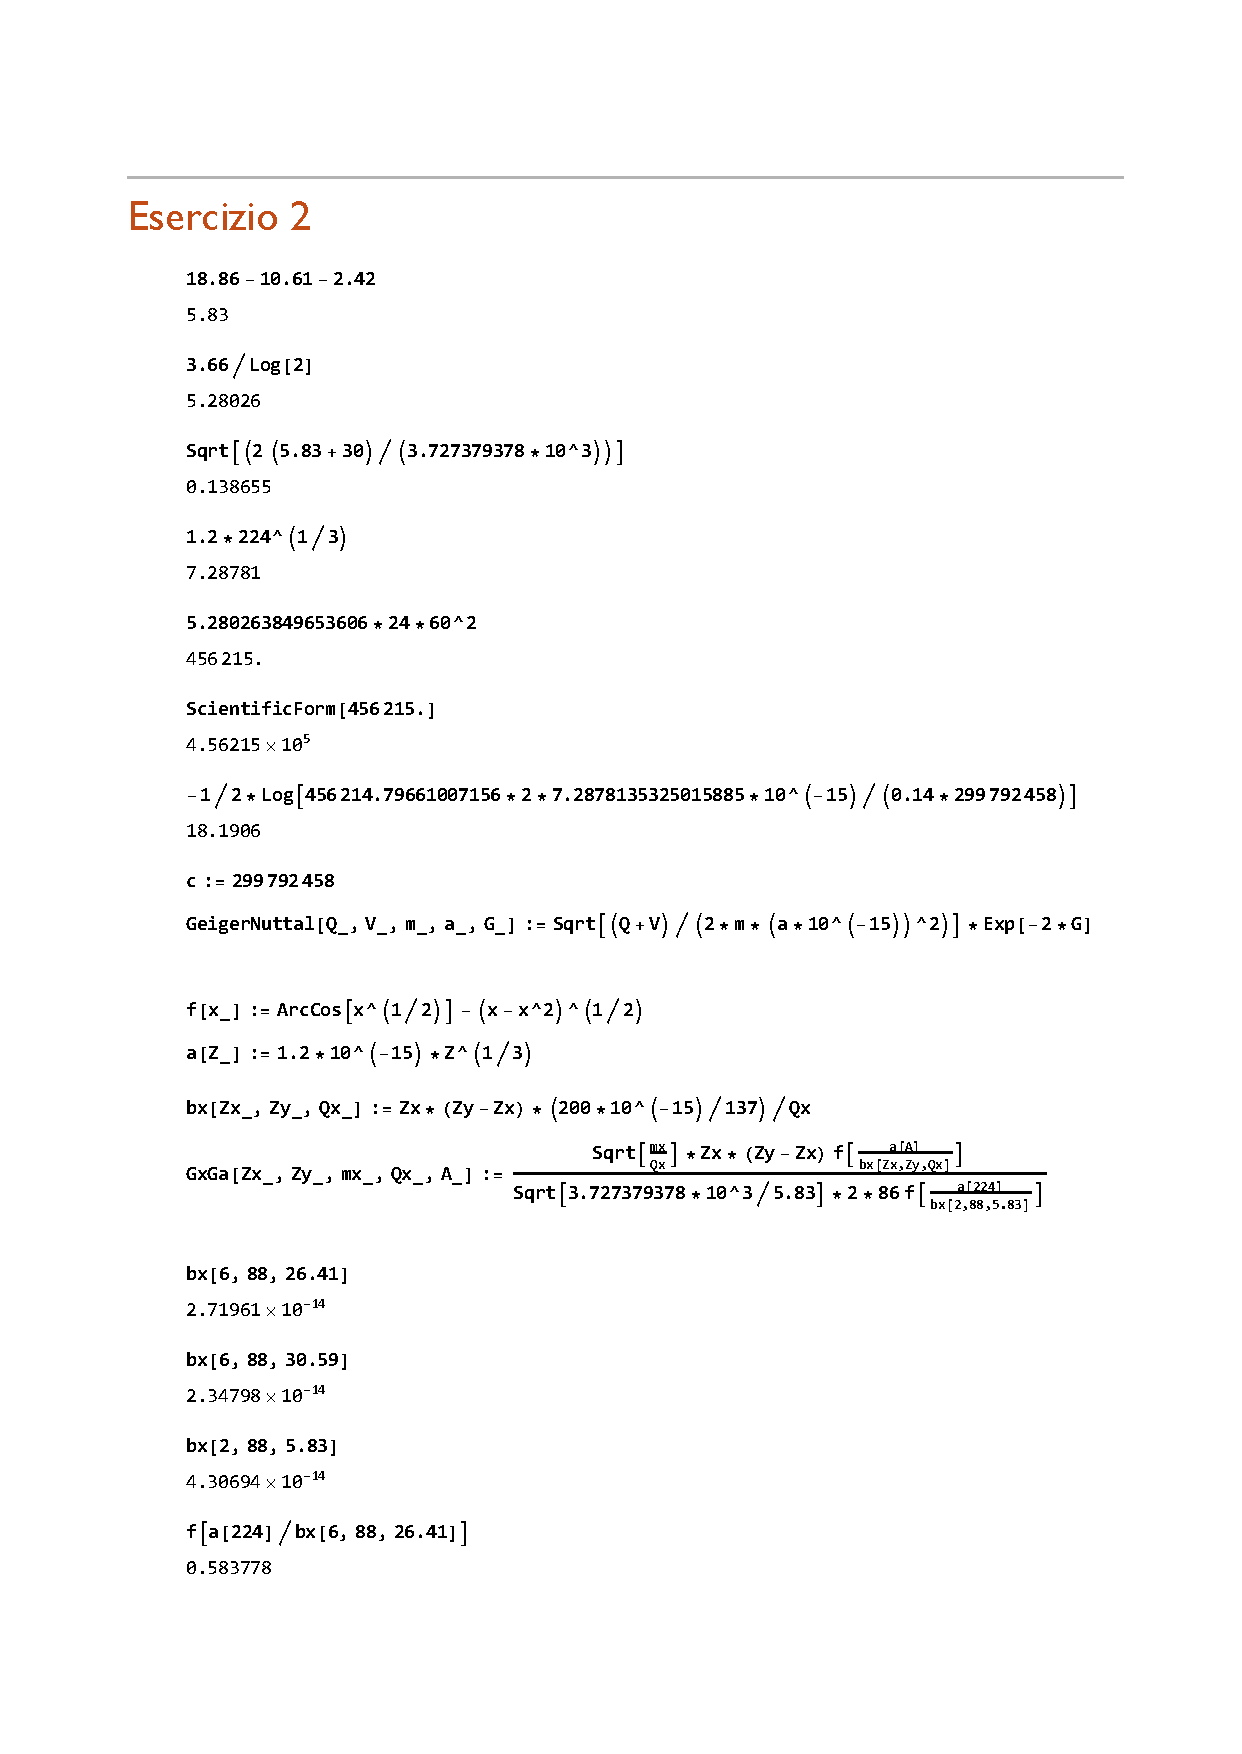
\includepdf{Conti/Esercizio2.pdf}
		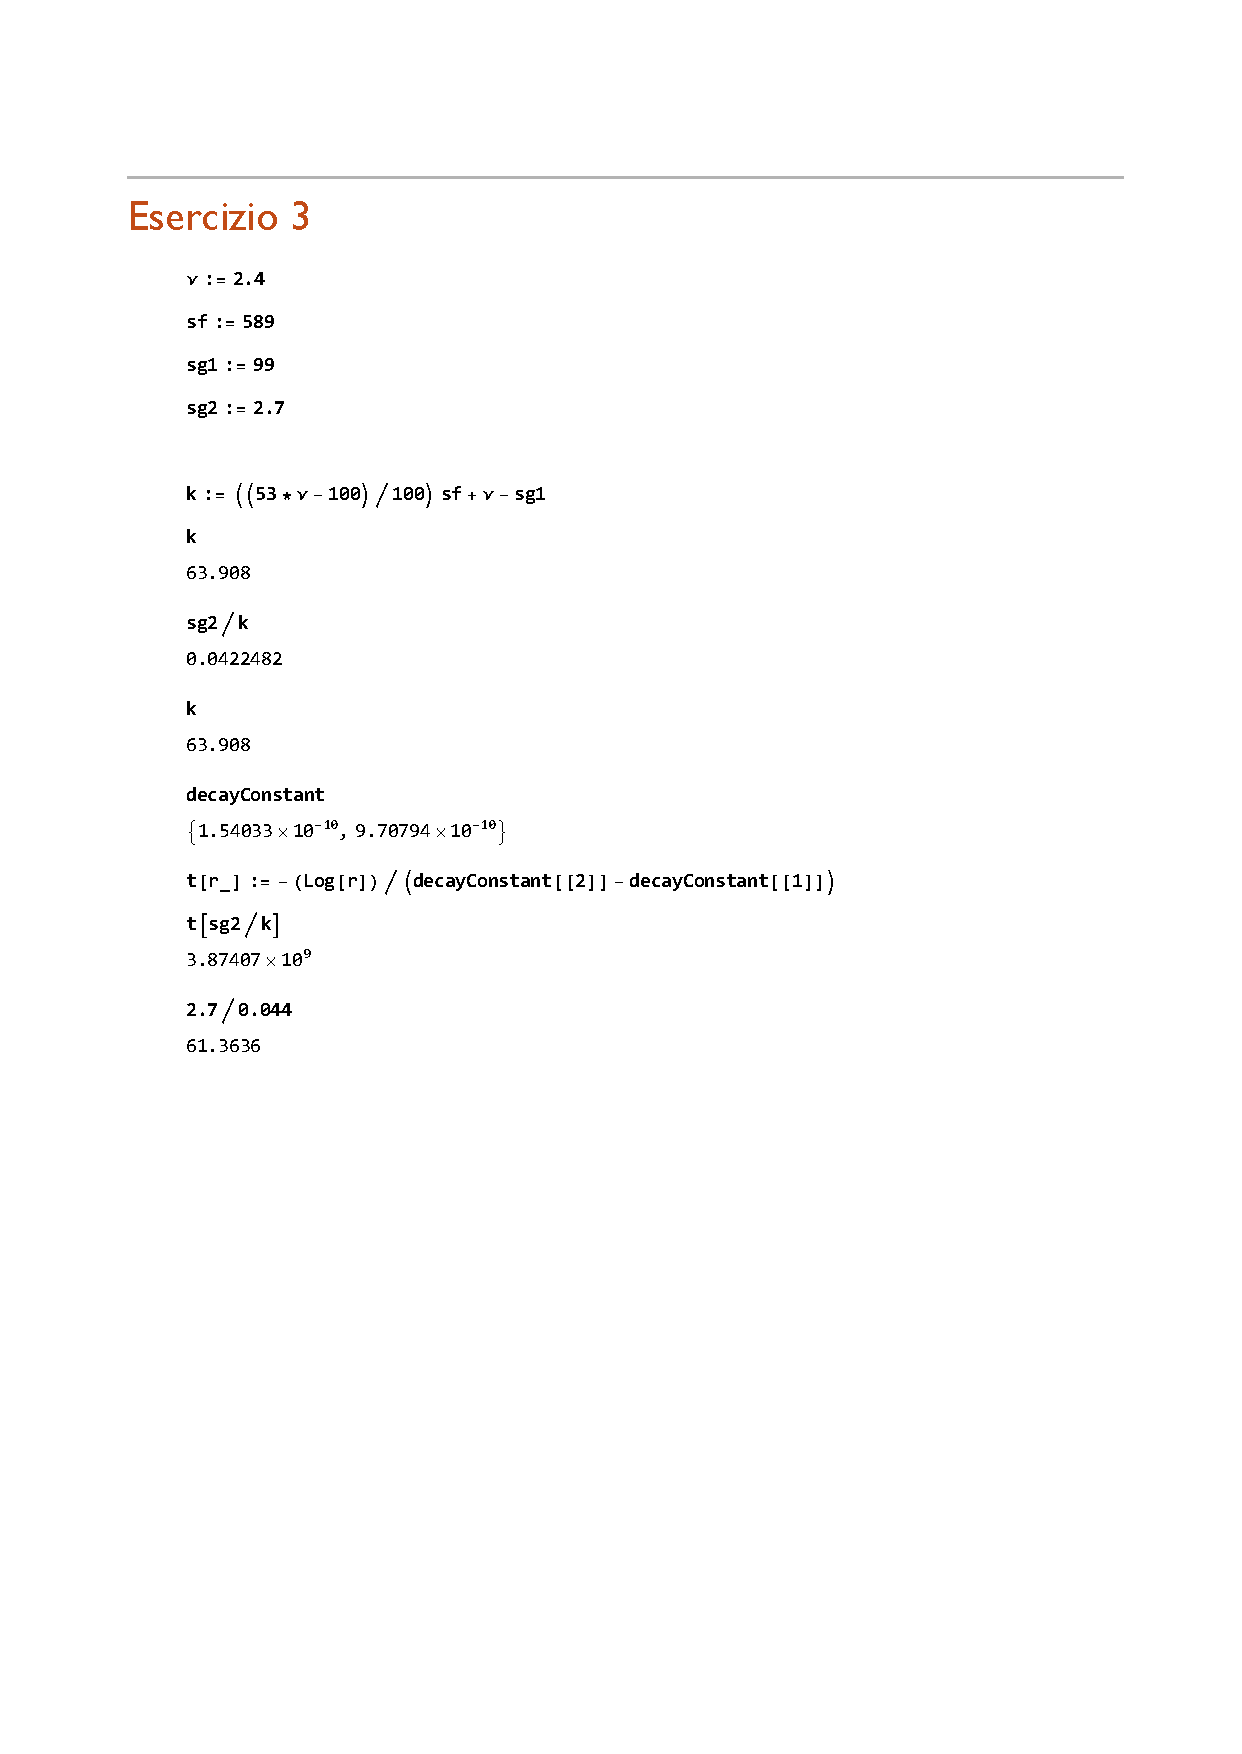
\includepdf{Conti/Esercizio3.pdf}
		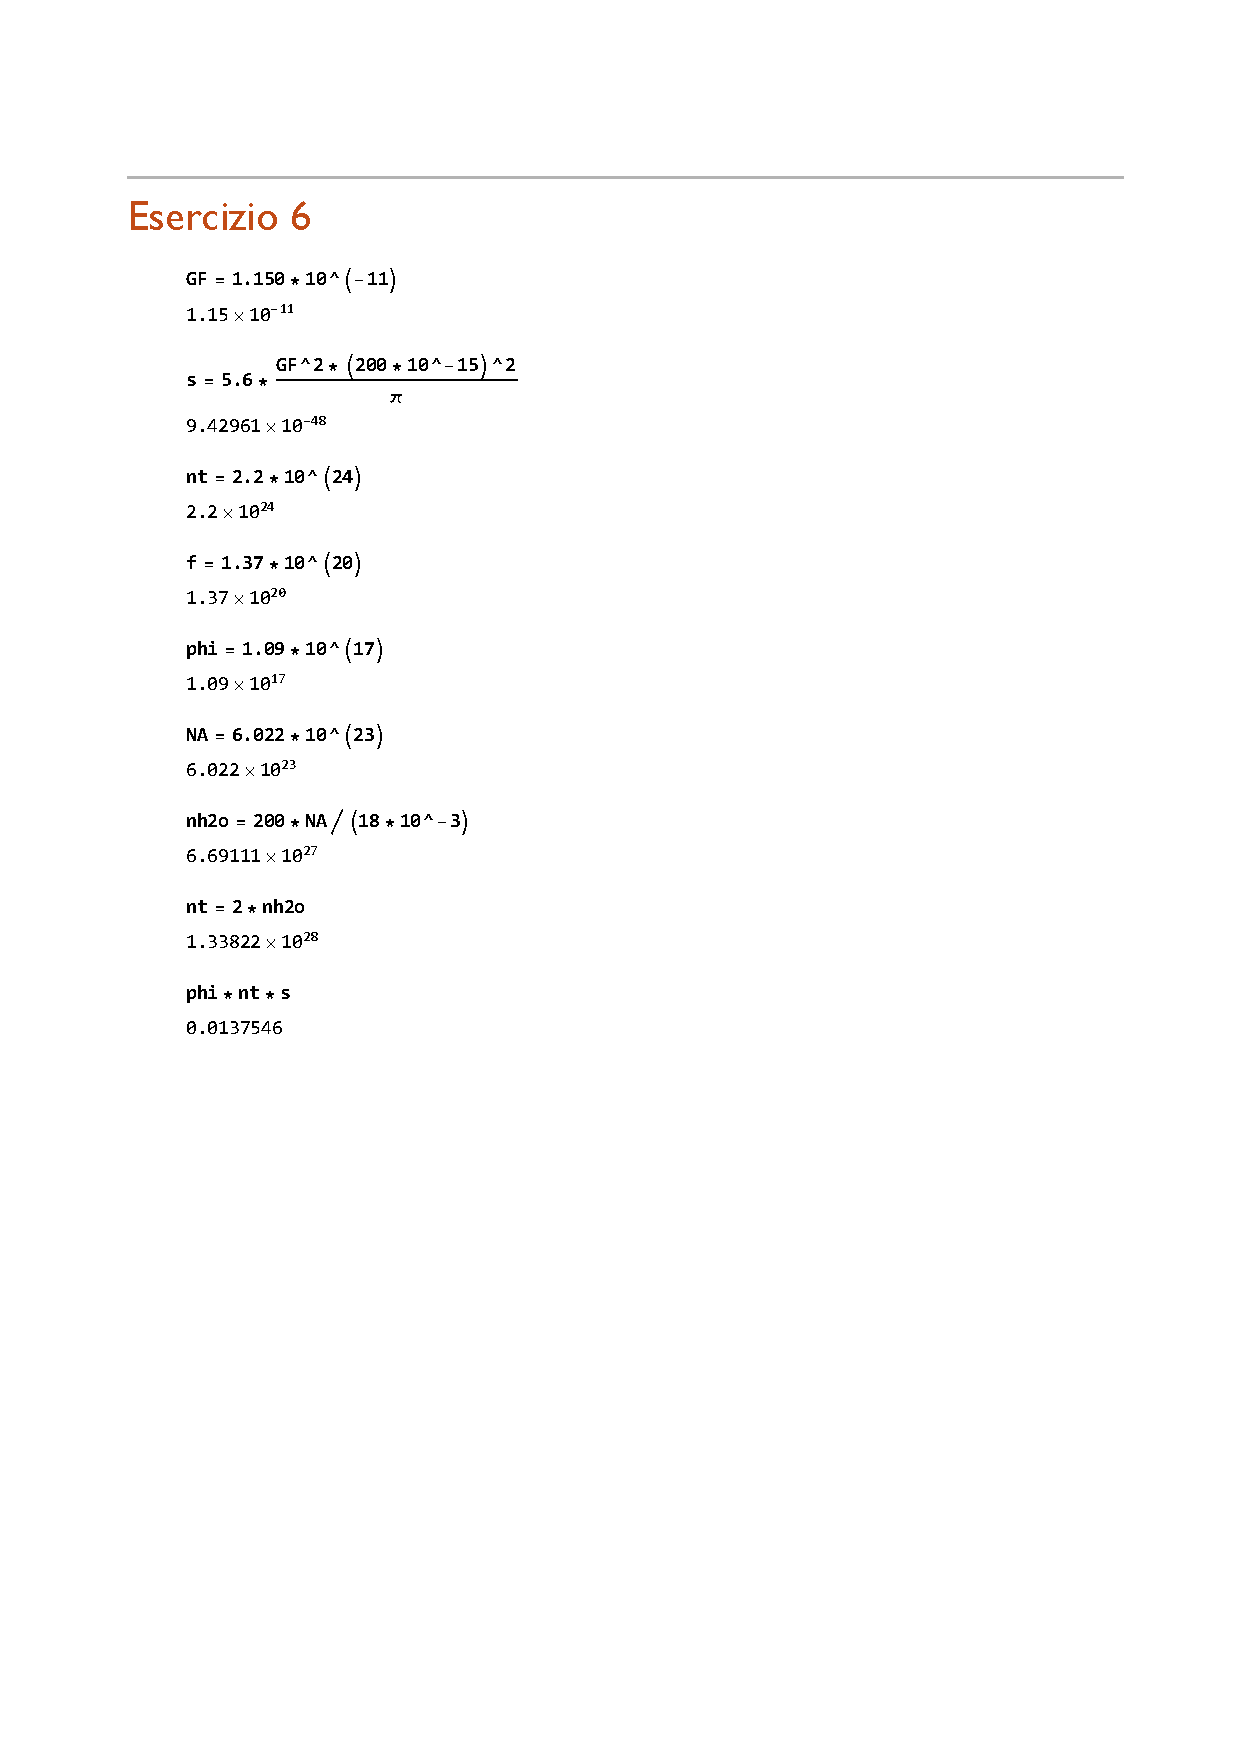
\includepdf{Conti/Esercizio6.pdf}
		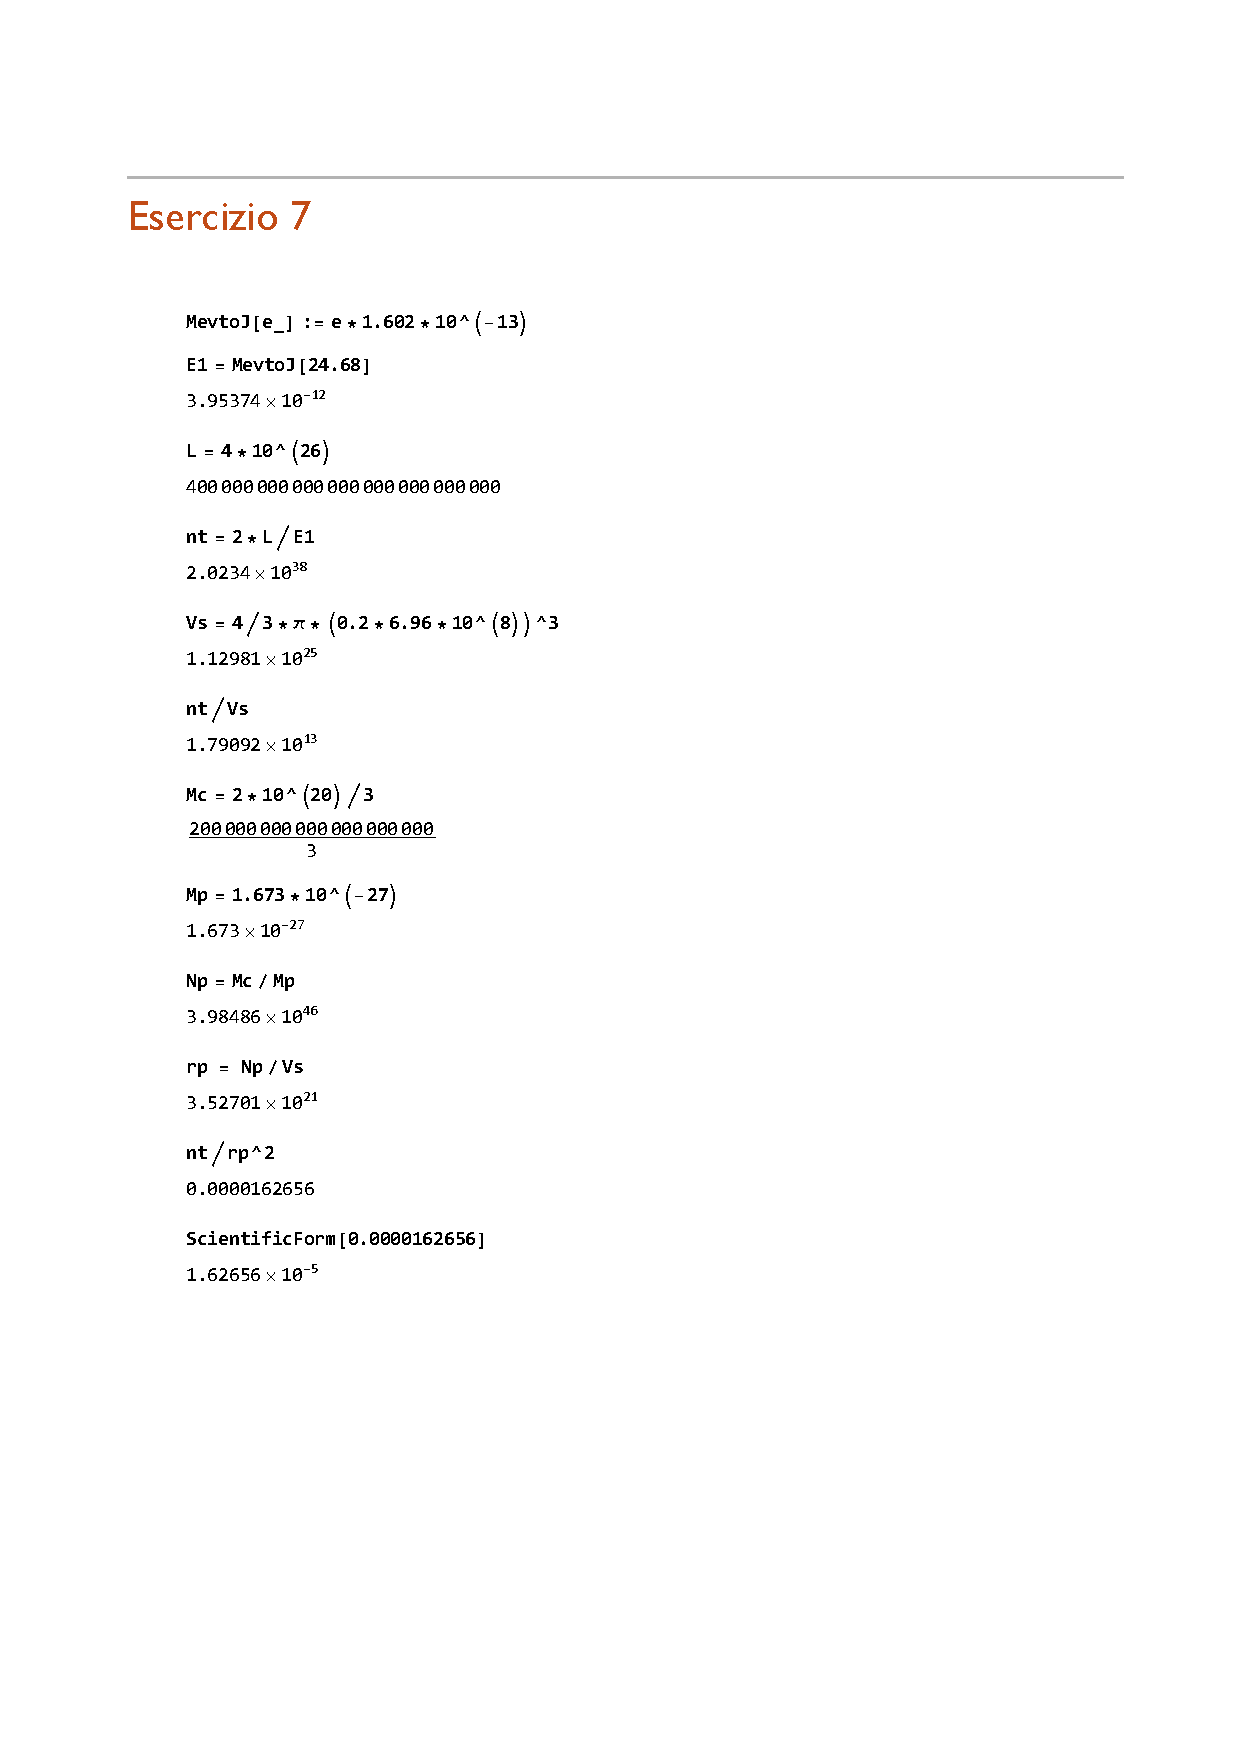
\includepdf{Conti/Esercizio7.pdf}
		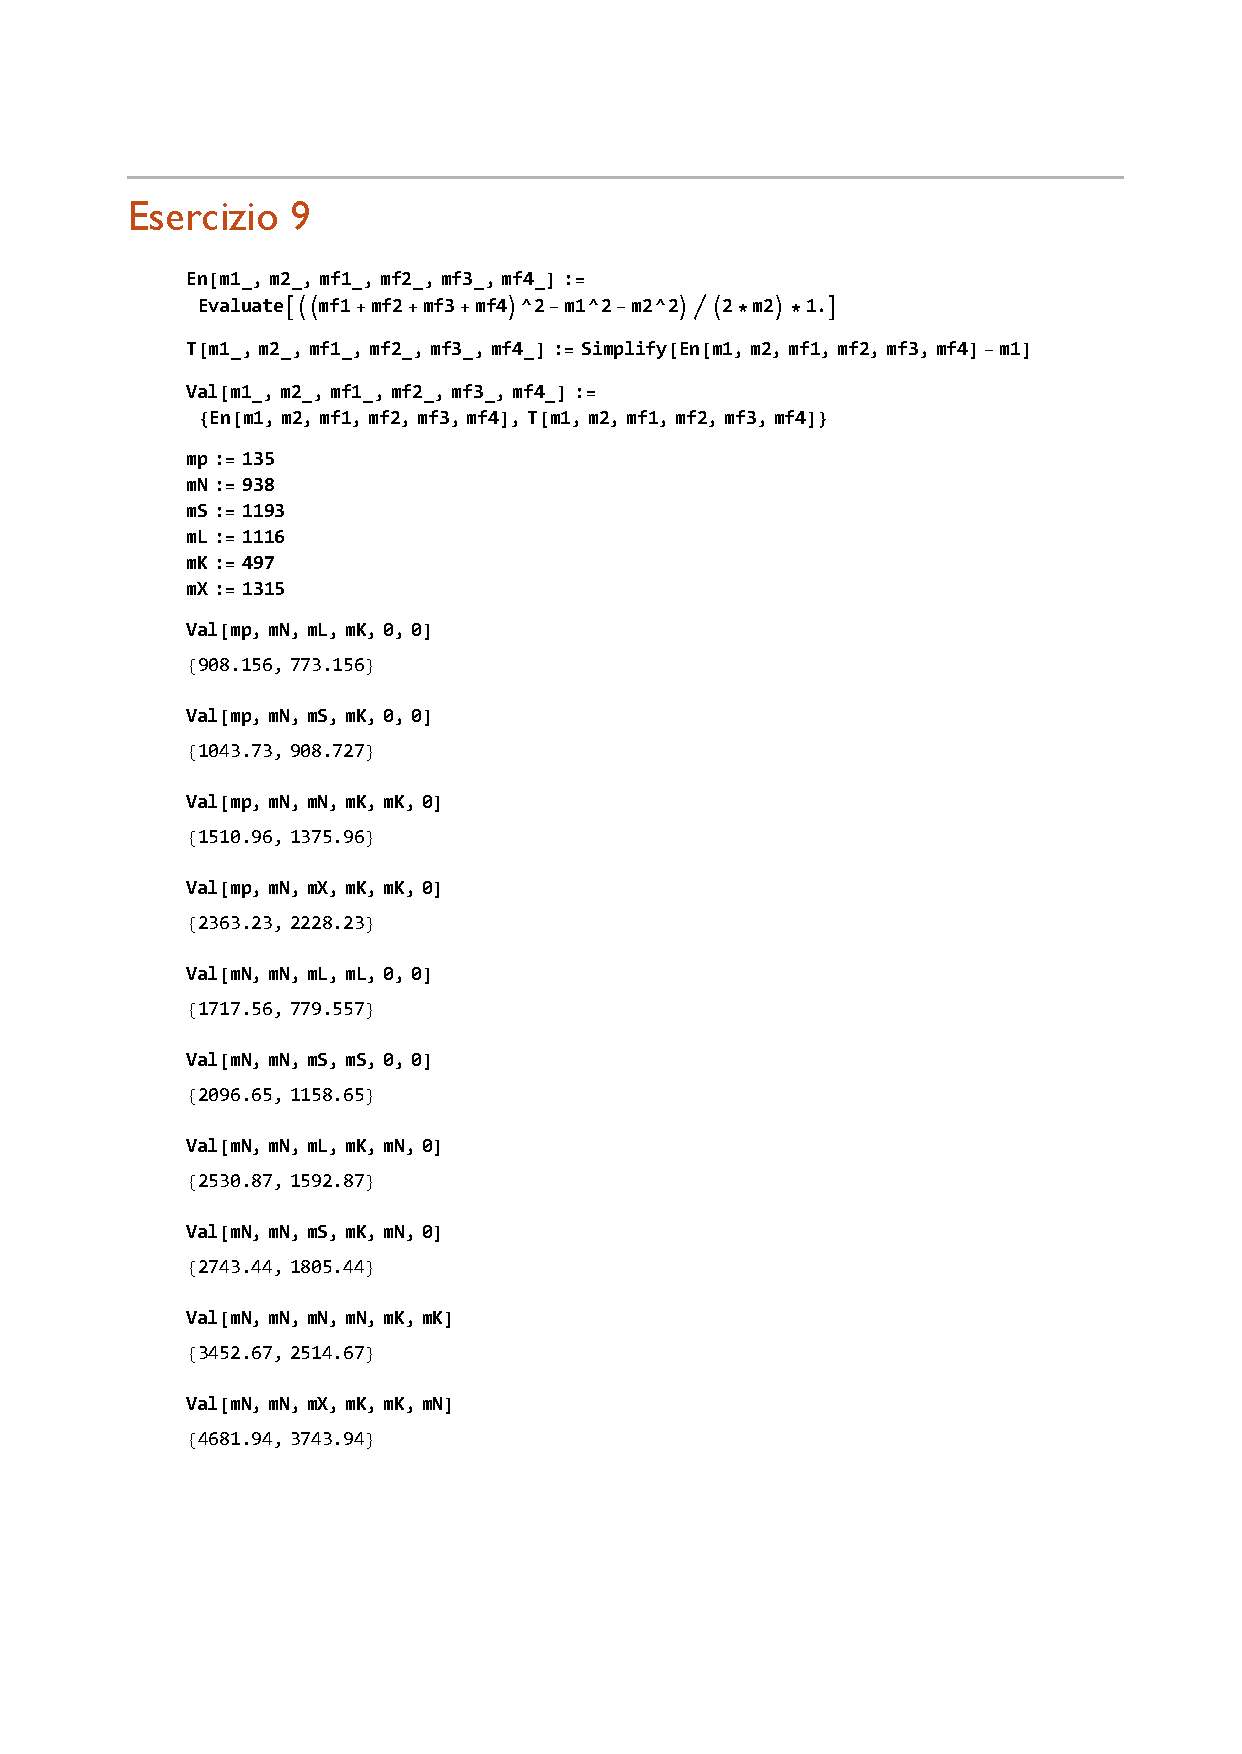
\includepdf{Conti/Esercizio9.pdf}
\end{document}